\chapter{Getting Started: New User with Existing Robot}\label{ch:getting_started}

This chapter will get a new user familiar enough with the PoliV2 platform that they will be able to:
\begin{itemize}
\item Create their own user accounts on PoliV2 computers
\item Turn on the robot and auxiliary systems
\item Start necessary robot services on their own user account(s)
\item Network their own PC to network into the roscore of the robot
\end{itemize}
It will be helpful to have a high level understanding of the robot and its systems. Before continuing, please look over Chapter \ref{ch:overview}.



\section{Turning on the hardware} \label{sec:turn_on_hardware}
The Segway RMP base contains two batteries- one for base propulsion and one for auxiliary systems. Both are activated and charged in parallel, making turn on and turn off procedures simple. Many components, like the router, pillar and lidar, will be powered up without direct intervention.

\subsection{Turning on the robot}
There are four main components that need to be powered manually. These are 
\begin{itemize}
	\item The Segway base
    \item The two PCs
    \item The Kinova arm
\end{itemize}

\subsubsection{The Segway base}
Locate the base control box, containing the power button and an Emergency-Stop button (Figure \ref{fig:base_powerbox}. Pressing the power button initiates the base's power up sequence or power down sequence, depending on the base's initial state.

\begin{figure}[h]
  \centering
  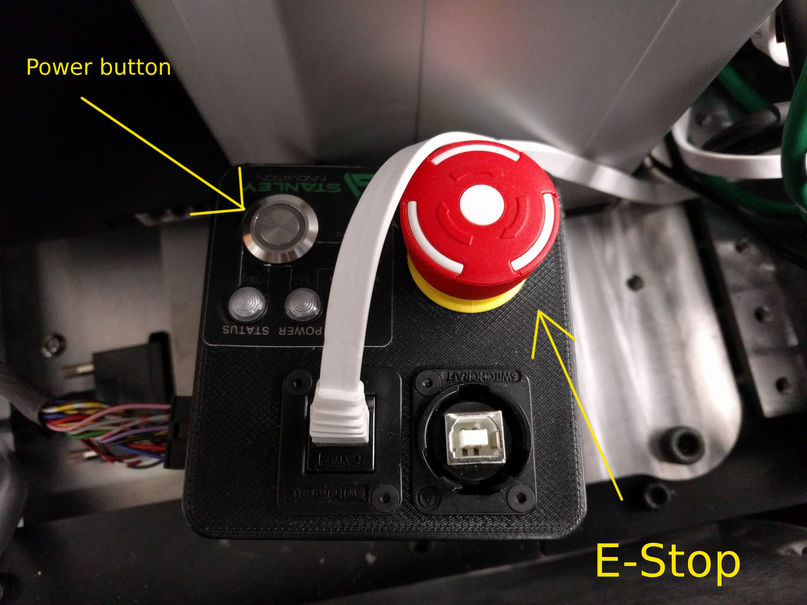
\includegraphics[width=300px]{figures/base_power.jpg}
  \caption{The Segway base control box}
  \label{fig:base_powerbox}
\end{figure}

During boot up and boot down, the base emits a tone that lets you know systems are normal. You can also verify the lights on the control box. 

\begin{figure}[h] 
  \centering
  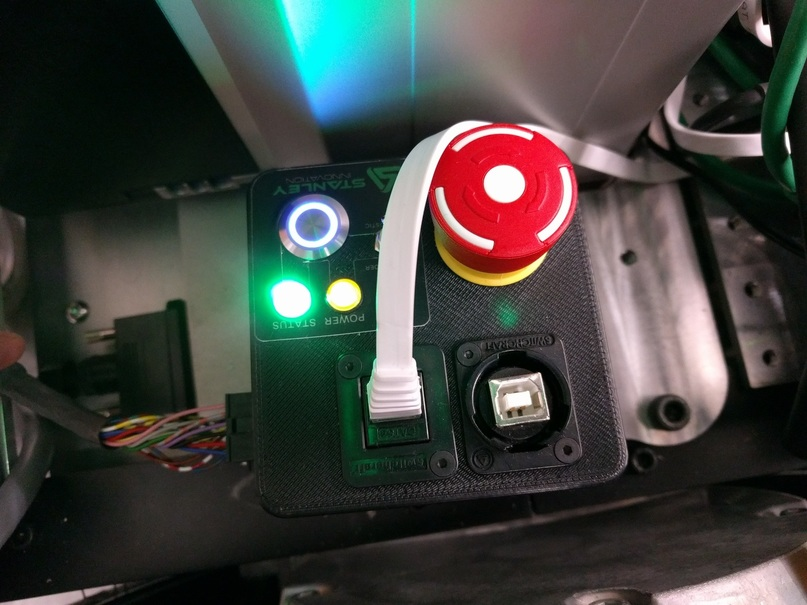
\includegraphics[width=300px]{figures/base_power_on.jpg}
  \caption{The control box power button is pulsing slowly and the indication LED is green. Both indicate system has booted normally.}
  \label{fig:base_powerbox_on}
\end{figure}

\subsubsection{PCs- Poli1 and Poli2}
The PCs also turn on at the press of a button. Since they use power supplied by the base, the base must already be turned on before attempting to power the PCs.\\

See Figure \ref{fig:computer_1_power} and Figure \ref{fig:computer_2_power} for help finding the power buttons. The power button on each computer should light up once powered.

\begin{figure}[h] 
  \centering
  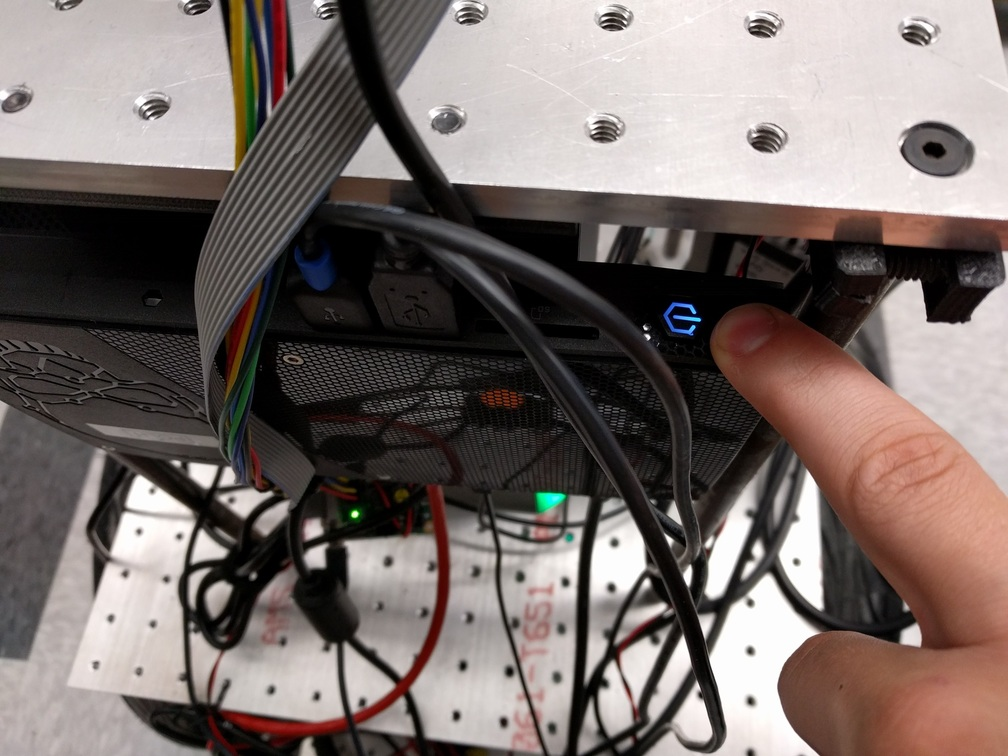
\includegraphics[width=300px]{figures/computer_1_power.jpg}
  \caption{Location of the power button for PC1.}
  \label{fig:computer_1_power}
\end{figure}

\begin{figure}[h] 
  \centering
  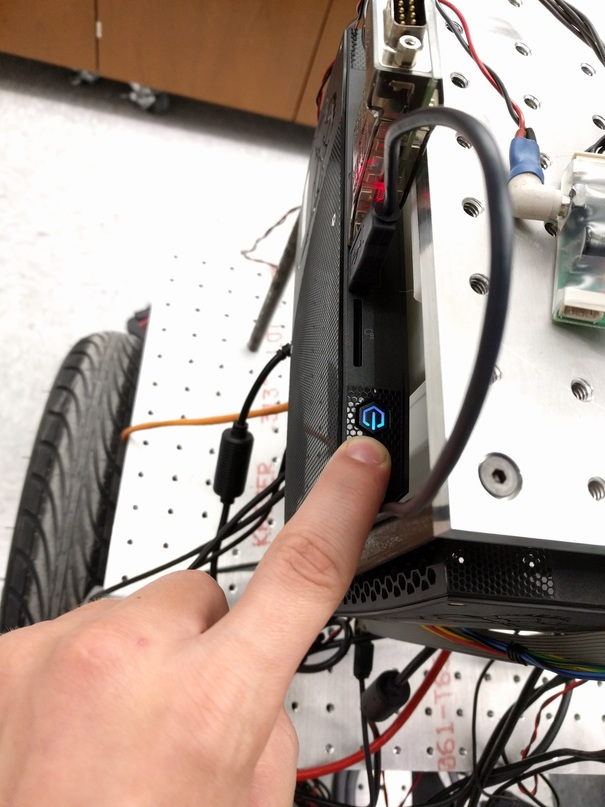
\includegraphics[height=300px]{figures/computer_2_power.jpg}
  \caption{Location of the power button for PC2.}
  \label{fig:computer_2_power}
\end{figure}

\clearpage

\subsubsection{Arm}
Since the arm is back-drivable when unpowered, it is sometimes advantageous to turn the arm off manually and move it to a safe position. If the previous operator has done this, you will want to check if the arm's power button is active. \\

Locate the arm's access panel- with power and USB inputs. The power button also exists on this panel. The arm is powered if you cannot move it or if its holding its own weight without falling.

\begin{figure}[h!] 
  \centering
  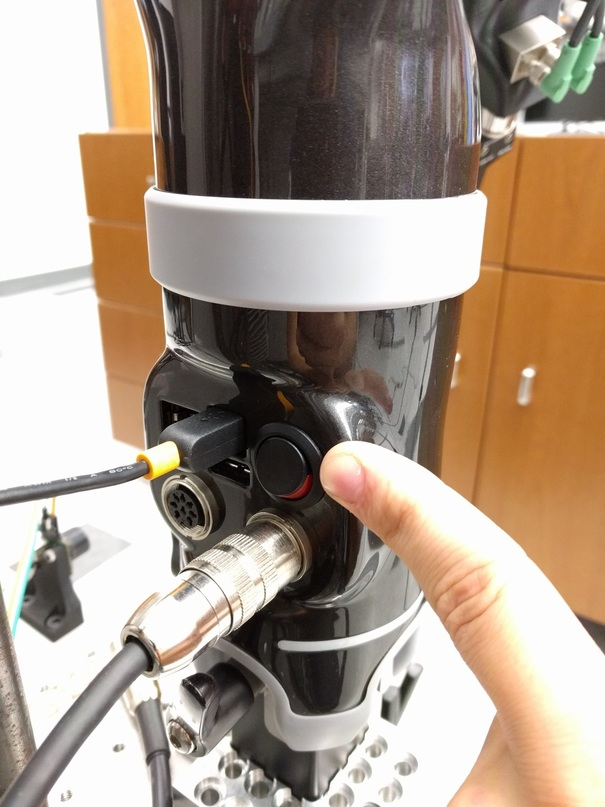
\includegraphics[height=300px]{figures/arm_power.jpg}
  \caption{Location of the power button for the Kinova Jaco2. In this case, the arm is on.}
  \label{fig:arm_power}
\end{figure}

\subsection{Turning off the robot}
This basically happens in the reverse sequence of turning the robot on. \\

First you should confirm the safety of the arm position and turn it off manually if necessary. See Figure \ref{fig:arm_power} for the power button location. \\

Secondly, the PCs should be soft-shutdown, if possible. This means running the \texttt{sudo shutdown now} command in a terminal in a ssh session with the PC. If necessary, you can hold down the power button to shut the PC down. \\

Lastly, press the base's powerbutton on its control box. An audible tone should sound, and the LED should blink red. It will be fully powered down in around a minute.

\subsection{Charging the robot}\label{sec:charging_robot}
The robot charges through a high voltage, VGA style connection directly into the base (see Figure \ref{fig:base_charger}). The cable is held into the base through two thumb-screws.

\begin{figure}[h!] 
  \centering
  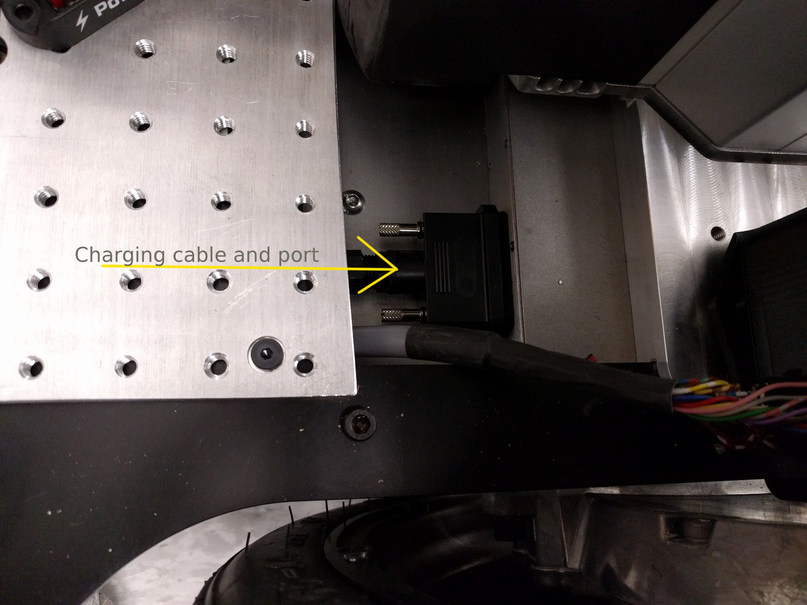
\includegraphics[width=250px]{figures/base_charging_cable_top.jpg}
  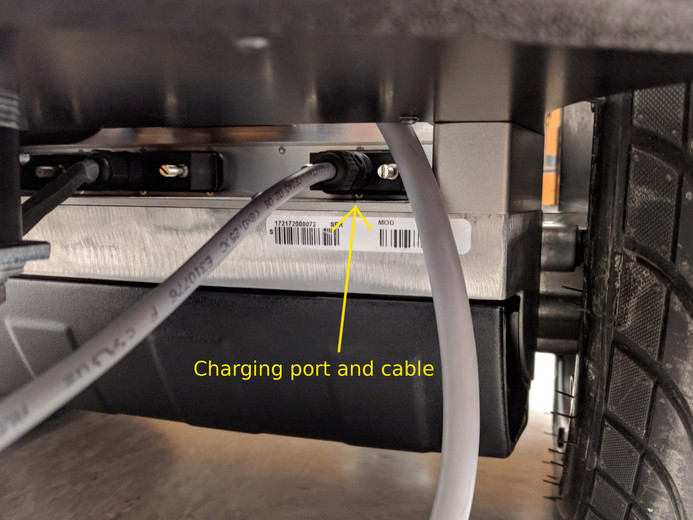
\includegraphics[width=250px]{figures/base_charging_cable_bottom.jpg}
  \caption{Top and bottom view of the charging cable connector for the Segway RMP.}
  \label{fig:base_charger}
\end{figure}

\clearpage

\textbf{\textcolor{red}{NOTE}} It is important that the charger be turned \textbf{OFF} when un/plugging the charging cable to the base. It is also important than the cable be inserted evenly, and not at an angle. Either of these can cause a momentary short and can tax the charger.

\begin{figure}[h!] 
  \centering
  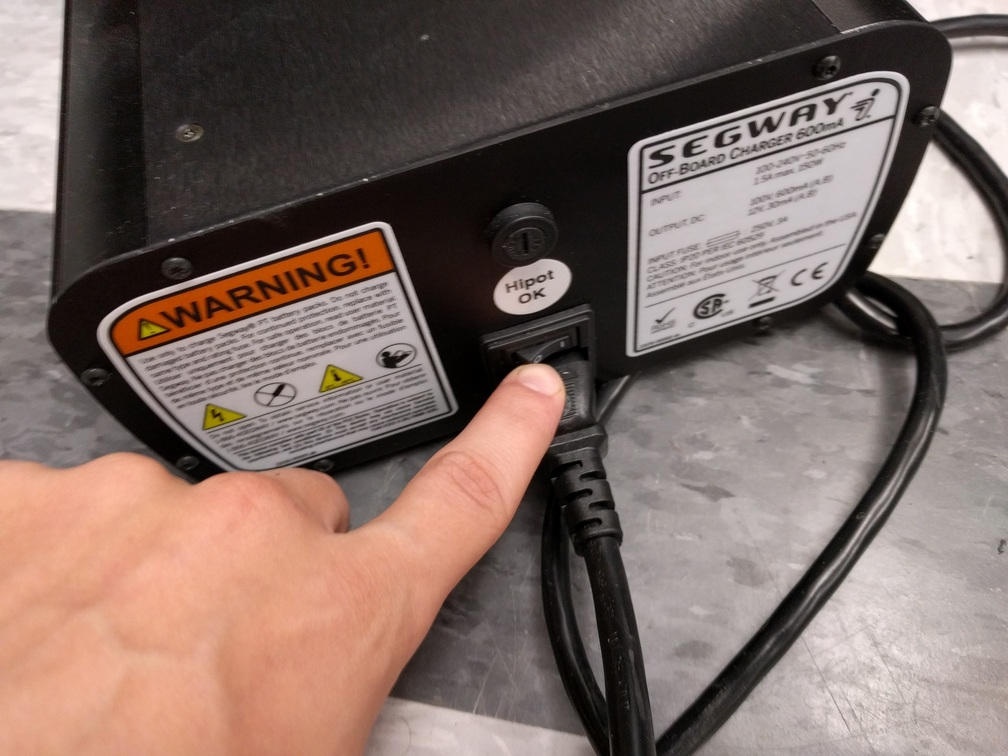
\includegraphics[width=250px]{figures/base_charger_turn_on.jpg}
  \caption{Back view of the Segway base charger. The charger's power switch is indicated.}
  \label{fig:base_charger_power}
\end{figure}

\subsection{Disconnecting robot from charger}
Turn the charger off using its power switch on its back panel. Unthread the thumb screws from the connector and the base. Pull the charging cable backwards, off the connector, with even force.

See Figure \ref{fig:base_charger} and Figure \ref{fig:base_charger_power} for details. 


\section{Create user accounts}\label{sec:user_accounts}
\subsection{Setting up local hosts file}
Examples in this section make use of a hostname alias, rather than specifying the IP address of \textbf{poli1}. 
To add \textbf{poli1} and \textbf{poli2} as hostnames, see Example \ref{ex:host_file}. 
This should already be done on the robot's computers but will need to be done for any computer used to access the robot's computers or network. 

\begin{example}{Example of setting hosts file for robot use}
  \label{ex:host_file}
  On your local computer (assuming Ubuntu)
  \begin{itemize}
    \item Open \texttt{/etc/hosts} with sudo privileges 
	\item Add \texttt{10.66.171.91 poli1}
    \item Add \texttt{10.66.171.24 poli2}
    \item Save and exit
  \end{itemize}
  IP addresses are assumed to be set according to Section \ref{sec:network_configuration}
\end{example}

\subsection{Initial Account Setup}
Connect to the robot's wireless network, which should be of the form \texttt{PoliV2-N}, where N is a number designating the enumeration of that particular robot. It is brought up when the router boots, which takes a couple minutes after turning on the robot. Since the robot needs to be powered for this, go ahead and look through Section \ref{sec:turn_on_hardware} to turn the robot on. \\

You can connect to the network using the password \textbf{simachines}. 
This same password is used for access to the default accounts on \textbf{poli1} and \textbf{poli2} computers.

We will now go through the process of adding a user account with the correct permissions to one of the PCs, \textbf{poli1}.

\begin{example}{Example of setting up user account on poli1}
  \label{ex:user_accounts}
  \begin{itemize}
  	\item ssh into poli1: \texttt{ssh poli@poli1}
    \item Make yourself a user: \texttt{sudo adduser <your desired username>}
    \item Add user to groups: \texttt{sudo usermod -aG sudo,dialout,cdrom,adm,dip,plugdev,lpadmin,sambashare,audio <your username>}
	\item  Log off: \texttt{exit}
    \item Set up your ssh keys for your new user: \texttt{ssh-copy-id <your user>@poli1}
	\item Log in to your new user account: \texttt{ssh <your user>@poli1}
  \end{itemize}
\end{example}

Now, log into your account and create a catkin workspace in your home directory. You can see how to do that at \\
\href{http://wiki.ros.org/catkin/Tutorials/create_a_workspace}{http://wiki.ros.org/catkin/Tutorials/create\_a\_workspace}.

If successful, do the same processes for \textbf{poli2}. Don't forget to setup your bash environment as in Example \ref{ex:bashrc_poli1}, \ref{ex:bashrc_poli2}.\\

\begin{example}{Setting up initial .bashrc file: POLI1}
  \label{ex:bashrc_poli1}
    Open \texttt{\textasciitilde/.bashrc} \\
    At the bottom add \texttt{source \textasciitilde/catkin\_ws/devel/setup.bash} \\
    Save and close \\
    In a terminal enter the command: \texttt{source \textasciitilde/.bashrc}
\end{example}

\begin{example}{Setting up initial .bashrc file: POLI2}
  \label{ex:bashrc_poli2}
    Open \texttt{\textasciitilde/.bashrc} \\
    At the bottom add \texttt{source \textasciitilde/catkin\_ws/devel/setup.bash} \\
    At the bottom add \texttt{source poli\_RMP.bash} \\
    At the bottom add \texttt{export ROS\_MASTER\_URI=http://poli1:11311} \\
    Save and close \\
    In a terminal enter the command: \texttt{source \textasciitilde/.bashrc}
\end{example}

Finally, you need to setup wireless internet under your user on \textbf{poli1} and \textbf{poli2}. 
This requires logging in by connecting a keyboard, mouse and monitor directly to the robot and setting up a connection to a network through Ubuntu's \texttt{network manager}. \\

There exist specific WiFi accounts for the robots to connect to the \texttt{utexas} network. Contact a lab manager for these credentials.

If \texttt{network manager}'s front face is updated to be X-forwarded or you switch to a different manager, you may be able to set up the wifi connection in a terminal via \texttt{ssh}.


\section{Setting up the code base}
\textbf{Note: This section of the guide is possibly outdated. Please see \href{https://github.com/si-machines/poli2/wiki}{the software wiki} for the latest.} \\

There are a fair number of forks and specific branches that need to be checked out to get all systems working.
Luckily the ROS-install system makes fetching these simple.

\subsection{Fetch high level repository}

\begin{example}{Setting up the PoliV2 codebase}
  \label{ex:poli2_codebase_setup}
  Assuming catkin\_ws is initialized and using a PoliV2 computer. \\
  \begin{itemize}
    \item \texttt{git clone https://github.com/si-machines/poli2.git} in \texttt{src} of catkin\_ws
    \item cd into root of \texttt{catkin workspace}
    \item \texttt{rosdep update}
    \item \texttt{rosdep install -{}-from-paths src -{}-ignore-src -{}-rosdistro=kinetic -y}
    \item \texttt{cd \textasciitilde/catkin\_ws/src} 
	\item \texttt{wstool init ./ ./poli2/dependencies.rosinstall}
    \item \texttt{sudo apt-get purge ros-kinetic-dynamixel-workbench-toolbox}
    \item \texttt{cd \textasciitilde}/catkin\_ws
    \item \texttt{catkin\_make}
  \end{itemize}
  In the future you can update from all repos using the \texttt{wstool update} command.
\end{example}


We use \texttt{rosdep} to fetch packages on the public repository list (reading from \texttt{package.xml}) and \texttt{wstool} to fetch specific branches of specific forks as specified in the \texttt{.rosinstall} file.

Note that the codebase should be set up on both \textbf{poli1} and \textbf{poli2}, so repeat Example \ref{ex:poli2_codebase_setup} on both PCs. \\

\textcolor{red}{Important note:} The last thing needed is to copy the \texttt{poli\_RMP.bash} file to the root of your home directory. 
This file is required by the \texttt{segway\_ros} driver. \\
As long as Examples \ref{ex:setup_rmp_env} and \ref{ex:bashrc_poli2} have been followed, the RMP environment variables should be set in perpetuity. 

\begin{example}{Setup RMP Environment Variables}\label{ex:setup_rmp_env}
\begin{itemize}
  \item \texttt{roscd poli\_launch}
  \item \texttt{cp config \textasciitilde/poli\_RMP.bash }
  \item \texttt{source \textasciitilde/.bashrc}
\end{itemize}
\end{example}



\section{Starting ROS and critical systems}
Since PoliV2 is a multi-purpose research platform, and will be used by many separate users, there are no assumptions made about the virtual environment.
As such, no \textit{\textbf{device}} launch files are brought up on startup or log-in; though the ability to do this is fully supported. See 'Automating Bringup Procedure` Section on the \href{https://github.com/si-machines/poli2/wiki/How-To}{Poli2 Wiki}.\\


However, a single launch file is brought up on startup to start the \textbf{ros core}. This is to prevent accidental preemption of the core, and to allow some (typically) persistent parameters to remain on the roscore session, e.g. robot\_description. \\



Thus, with the robot's systems on and the codebase installed and compiled, we're ready to bring up the systems manually.

\subsection{Poli1 PC}
As detailed in Section \ref{sec:network_configuration}, each PC can only bring up the devices it has connected to it, plus any networked components. 

We can bring up all poli1's devices as in Example \ref{ex:poli1_bringup}.

\begin{example}{Bringup poli1's devices}
  \label{ex:poli1_bringup}
    \texttt{ssh user@poli1} \\
  \texttt{roslaunch poli\_launch poli1\_bringup.launch}
\end{example}

\subsection{Poli2 PC}
We can bring up all poli2's devices as in Example \ref{ex:poli2_bringup}.
\texttt{poli2\_bringup.launch} does the heavy lifting, bringing up the navigation stack, MoveIt!, and all networked components. \\

\begin{example}{Bringup poli2's devices}
  \label{ex:poli2_bringup}
  \texttt{ssh user@poli2} \\
  \texttt{roslaunch poli\_launch poli2\_bringup.launch} \\
  Wait several seconds \\
  \texttt{roslaunch poli\_launch scan\_merger.launch}
\end{example}

Note that you must launch the scan\_merger.launch file after bringing up everything else on \textbf{poli2}. 
This is due to a bug in the implementation of the scan merger node. 
However, it is still necessary to run, due to the navigation stack's reliance on the merged tf frame that the scan merger provides. Otherwise, issues with the tf tree ensue. \\

Now all the robot's systems should be up. If you run into problems, check the troubleshooting page on the \href{https://github.com/si-machines/poli2/wiki}{poli2 high level repository} or in Chapter \ref{ch:troubleshooting} of this document. You can see specific examples of how to move components or access robot state in Chapter \ref{ch:componentspecifics}.

\subsection{Networking the Robot With Your Computer}
This allows you to run graphical elements (RViz, image\_view, etc) on your local machine that may be difficult or impossible to view on the robot's computers directly. \\

\begin{example}{Reserving IP on the robot's network} \label{ex:reserve_ip}
\begin{itemize}
  \item On your PC, connect to the desired robot's WiFi
  \item Go to the router's webpage: \texttt{10.66.171.1}
  \item Login
  \item Click \textbf{Advanced}
  \item Under \textbf{Network} in the navigation pane, select \textbf{DHCP server}
  \item There will be a table of MAC addresses and IP addresses...
  \item Find the \textbf{name} entry of your host and click \textbf{bind}.
  \item Copy the IP address that your machine is bound to.
\end{itemize}
\end{example}

\begin{example}{Setting up ROS Environment}\label{ex:setting_up_bashrc}
\begin{itemize}
  \item Edit your \texttt{\textasciitilde/.bashrc} file
  \item At the bottom add \texttt{export ROS\_IP=xyz} where \texttt{xyz} is the IP your machine is bound to on the network.
  \item At the bottom add \texttt{export ROS\_MASTER\_URI=http://poli1:11311}
  \item Save and close
  \item Source your .bashrc: \texttt{source \textasciitilde/.bashrc}
\end{itemize}
  In the event you want to run a roscore locally, simply change this file again, but where \texttt{ROS\_IP=127.0.0.1} and \texttt{ROS\_MASTER\_URI=http://localhost:11311}.
\end{example}

Example \ref{ex:reserve_ip} walks through binding your IP, which prevents getting kicked off the ROS network when your IP lease expires. 
Example \ref{ex:setting_up_bashrc} walks through setting up the environment variables needed to network through the robot. \\

Note that this would have to be done on each robot you want to work with, since each has its own network. 
Therefore it will be easier to reserve the same IP address on each robot network, preventing you from needing to update your \texttt{\textasciitilde/.bashrc} with each new robot. \\


You can read more about ROS networking at \href{http://wiki.ros.org/ROS/NetworkSetup}{http://wiki.ros.org/ROS/NetworkSetup}.
